\documentclass[margin]{resphoto}  
\usepackage{helvet}
\usepackage{hyperref}
\usepackage{graphicx}
\usepackage{multirow}
\usepackage{enumitem,kantlipsum}

% 使用原生命令精准控制版面，彻底解决页脚太窄、报错的问题
\textheight=680pt        % 稍微缩短正文高度，给底部留出更多空间
\voffset=-0.2in          % 将整个版面稍微往上提一点点
\begin{document}

%-------------------------------------------------------------------------------
%	NAME AND ADDRESS SECTION
%-------------------------------------------------------------------------------
\name{\textbf{\LARGE Yang, Liu }}

% Note that addresses can be used for other contact information:
% -phone numbers
% -email addresses
% -linked-in profile

% Simulate as if there are 7 lines of address
\address{\\\\\\
            Title: Assistant Professor (Tenure Track)\\
            \qquad\quad Presidential Young Professor \\
            \qquad\quad Department of Mathematics \\
            \qquad\quad National University of Singapore
            \\\\
            Email: \url{yangliu@nus.edu.sg}\\\\
            Website: \url{https://scaling-group.github.io/}, \href{https://scholar.google.com/citations?user=3qRUYIYAAAAJ}{Google Scholar} \\\\
            }
% Hence the photo would take 7 lines/rows
% \address{\multirow{5}{*}{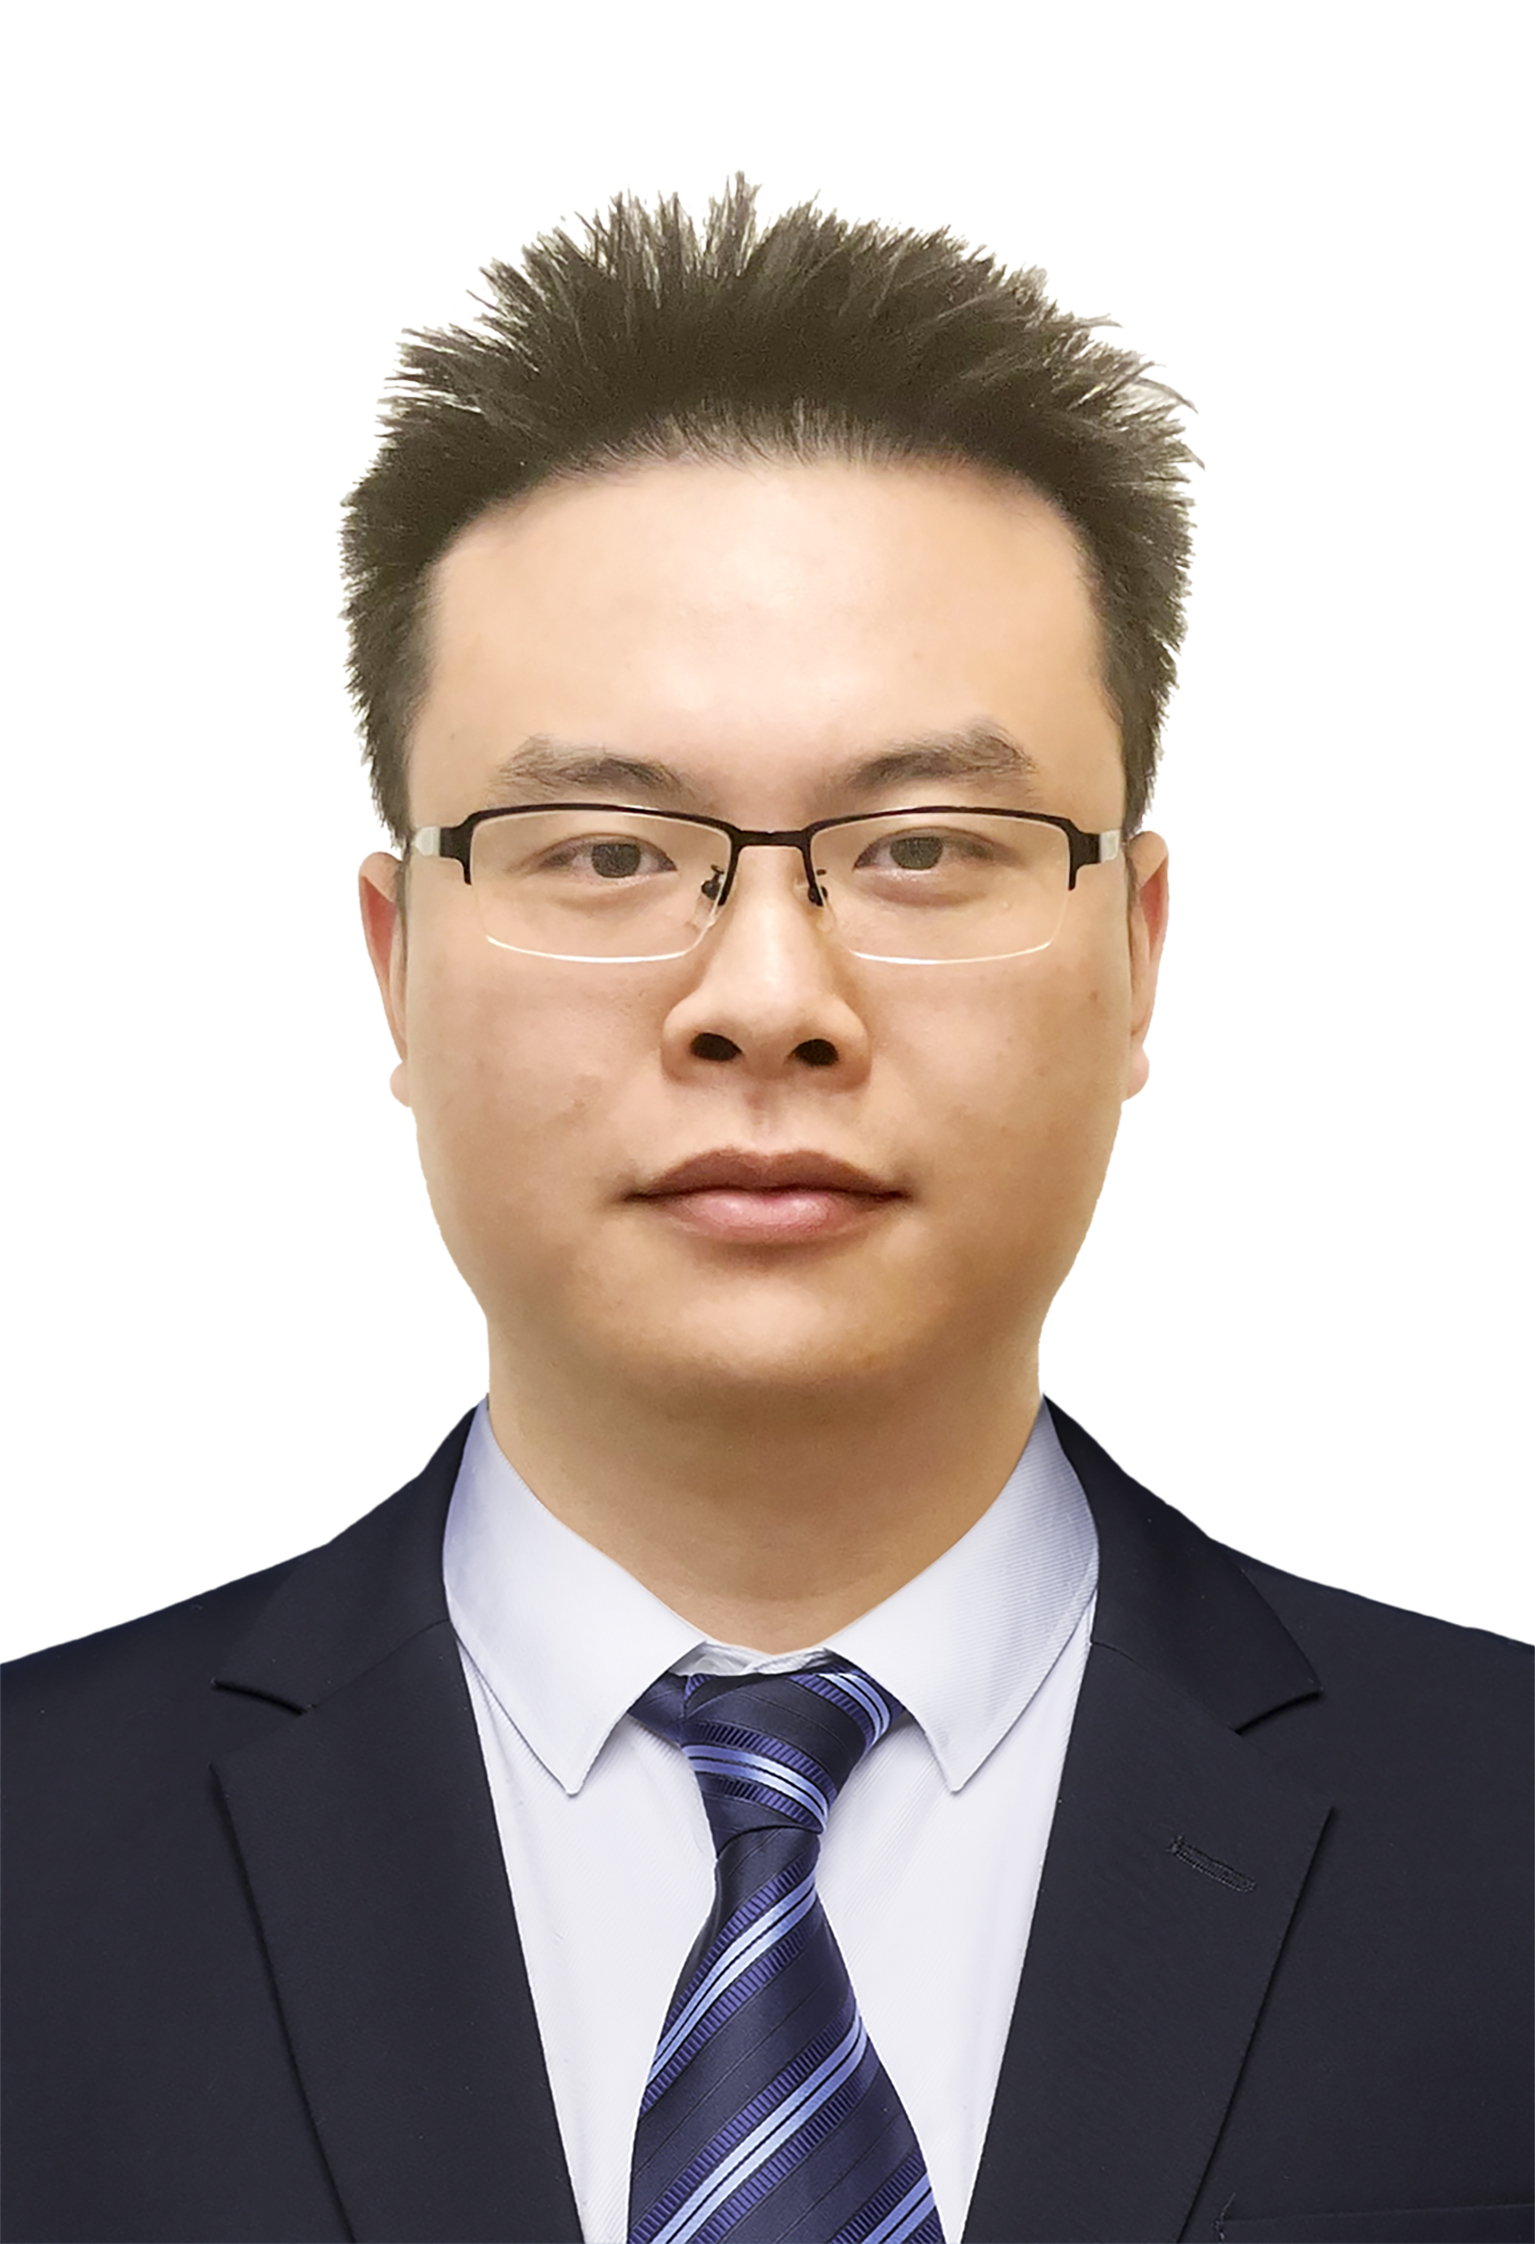
\includegraphics[width=2.8cm]{photo.jpg}}\\}

% Uncomment to add a third address
%\address{Address 3 line 1\\Address 3 line 2\\Address 3 line 3}
%-------------------------------------------------------------------------------

\begin{resume}

%-------------------------------------------------------------------------------
%	EDUCATION SECTION
%-------------------------------------------------------------------------------
\section{EDUCATION}

\textbf{Brown University}, Providence, RI, USA\\
Ph.D. in Applied Mathematics, May 2021\\
Sc.M. in Applied Mathematics, May 2018\\
Advisor: George Karniadakis\\
Dissertation: Generative Adversarial Networks for Physics-Informed Learning

\textbf{Tsinghua University}, Beijing, China\\
B.E. in Engineering Mechanics, July 2016\\
\href{https://www.hy.tsinghua.edu.cn/hyen/info/1176/1065.htm}{Tsien Hsue-Shen Elite Class in Mechanics}\\
Outstanding Graduate Honor (Top 10\%)


%-------------------------------------------------------------------------------
\section{WORK}
\textbf{National University of Singapore}, Singapore\\
Assistant Professor, Department of Mathematics, July 2024-present
\\Presidential Young Professor

\textbf{University of California, Los Angeles}, Los Angeles, CA, USA\\
Assistant Adjunct Professor, Department of Mathematics, July 2022-June 2024
\\Working with Prof. Stanley Osher.

\textbf{WeRide Corp}, San Jose, CA, USA\\
Software Engineer, June 2021-June 2022
\\Developing autonomous driving systems, with a focus on planning and decision-making in uncertain environments.

%-------------------------------------------------------------------------------
% \section{RESEARCH INTERESTS}
% \begin{itemize}[leftmargin=*]
% \item Build scalable AI for real-world challenges, including forward PDE solving, robotic control, inverse problems, etc.
% \item Answer some important fundamental questions in AI, including how to generalize from easy to hard tasks, how emergent capabilities arise, etc.
% \end{itemize}


\section{AWARDS}
\begin{itemize}[leftmargin=*]
\item Presidential Young Professorship, National University of Singapore (2024)
\item David Gottlieb Memorial Award, Brown University, USA (2021)
\item Outstanding Graduate Honor (Top 10\%), Tsinghua University, China (2016)
\item Scholarship for Academic Excellence, Tsinghua University, China (2013, 2015)
\item Tsien Hsue-Shen Elite Class in Mechanics, Tsinghua University, China (2012-2016)
\end{itemize}


\section{GRANTS}
\begin{itemize}[leftmargin=*]
\item Singapore National Research Foundation Fellowship, August 2025 - August 2030
\end{itemize}

%-------------------------------------------------------------------------------
\section{PUBLICATIONS \& PREPRINTS}
% \section{SELECTED PUBLICATIONS} % Citations over 7000, h-index 13, by April 2025\\
$*$ indicates equal contribution. $\dagger$ indicates corresponding author(s).

\begin{itemize}[leftmargin=*]
\item Chenghan Wu, Zongmin Yu, and {Liu Yang}$^\dagger$. ``A Foundation Model of Numerical Intelligence with Cross-Disciplinary Generalization'' \textit{arXiv:2607.28432} (2026).
\item Zongmin Yu, and {Liu Yang}$^\dagger$. ``Agentic Symbolic Search: Characterizing PDEs Beyond Hand-crafted Expressions, Meshes, and Neural Networks'' \textit{arXiv:2606.20467} (2026).
\item Minghui Yang, Ling Guo, and {Liu Yang}$^\dagger$. ``Harness In-Context Operator Learning with Chain of Operators'' \textit{arXiv:2606.12318} (2026).
\item Song Chen$^*$, Linyan Xiang$^*$, Ying Zhou, and {Liu Yang}$^\dagger$. ``VICX: Generalizable Robot Manipulation via Video Generation and In-Context Operator Network'' \textit{arXiv:2606.12028} (2026).
\item Boai Sun, Wenjin Guo, Zongmin Yu, and {Liu Yang}$^\dagger$. ``Self-Evolving Scientific Agent Discovers Generalizable Physically-Reasoned Fluid Control'' \textit{arXiv:2606.08405} (2026).
\item Zongmin Yu, and {Liu Yang}$^\dagger$. ``Evolving Ensemble of Agents'' \textit{arXiv:2605.09018} (2026).
\item Lingfeng Li$^*$, Zhuoyuan Li$^*$, Shun Li$^*$, Kaixin Zhan, Huajian Gao$^\dagger$, Changqing Chen$^\dagger$, and {Liu Yang}$^\dagger$. ``In-Context Modeling as a Retrain-Free Paradigm for Foundation Models in Computational Science'' \textit{arXiv:2604.23098} (2026).
\item Ziyang Liu$^*$, Xinyan Guo$^*$, Xuchen Wei$^*$, Han Hao$^\dagger$, and {Liu Yang}$^\dagger$. ``Escher-Loop: Mutual Evolution by Closed-Loop Self-Referential Optimization'' \textit{arXiv:2604.23472} (2026).
\item Chenghan Wu, Zongmin Yu, Boai Sun, and {Liu Yang}$^\dagger$. ``Graph In-Context Operator Networks for Generalizable Spatiotemporal Prediction'' \textit{arXiv:2603.12725} (2026).
\item Yadi Cao$^*$, Yuxuan Liu$^*$, {Liu Yang}, Rose Yu, Hayden Schaeffer, and Stanley Osher$^\dagger$. ``VICON: Vision In-Context Operator Networks for Multi-Physics Fluid Dynamics Prediction'' \textit{Transactions on Machine Learning Research} (2026).
\item Xinyu Ma, Chengxin Wang, Meng Wang, Xu Guo, {Liu Yang}$^\dagger$, and Huajian Gao$^\dagger$. ``Gaussian Ensemble Topology (GET): A New Explicit and Inherently Smooth Framework for Manufacture-Ready Topology Optimization'' \textit{arXiv:2510.05572} (2025).
\item {Liu Yang}, Siting Liu, and Stanley J. Osher$^\dagger$. ``Fine-Tune Language Models as Multi-Modal Differential Equation Solvers'' \textit{Neural Networks} (2025): 107455.
\item {Liu Yang}, and Stanley J. Osher$^\dagger$. ``PDE Generalization of In-Context Operator Networks: A Study on 1D Scalar Nonlinear Conservation Laws'' \textit{Journal of Computational Physics} 519 (2024): 113379.
\item {Liu Yang}, Siting Liu, Tingwei Meng, and Stanley J. Osher$^\dagger$. ``In-Context Operator Learning With Data Prompts for Differential Equation Problems'' \textit{Proceedings of the National Academy of Sciences} 120.39 (2023): e2310142120.
\item Xuhui Meng$^*$, {Liu Yang}$^*$, Zhiping Mao, José del Águila Ferrandis, and George Em Karniadakis$^\dagger$. ``Learning Functional Priors and Posteriors from Data and Physics.'' \textit{Journal of Computational Physics} 457 (2022): 111073.
\item {Liu Yang}, Constantinos Daskalakis, and George E. Karniadakis$^\dagger$. ``Generative Ensemble Regression: Learning Particle Dynamics From Observations of Ensembles with Physics-Informed Deep Generative Models'' \textit{SIAM Journal on Scientific Computing} 44.1 (2022): B80-B99.
\item {Liu Yang}, Tingwei Meng, and George E. Karniadakis$^\dagger$. ``Measure-Conditional Discriminator with Stationary Optimum for GANs and Statistical Distance Surrogates'' \textit{arXiv:2101.06802} (2021).
\item George Em Karniadakis$^\dagger$, Ioannis G. Kevrekidis, Lu Lu, Paris Perdikaris, Sifan Wang, and {Liu Yang}. ``Physics-Informed Machine Learning'' \textit{Nature Reviews Physics} 3.6 (2021): 422-440. (alphabetical order)
\item {Liu Yang}$^*$, Xuhui Meng$^*$, and George Em Karniadakis$^\dagger$. ``B-PINNs: Bayesian Physics-Informed Neural Networks for Forward and Inverse PDE Problems With Noisy Data'' \textit{Journal of Computational Physics} 425 (2021): 109913.
\item Xiaoli Chen, {Liu Yang}, Jinqiao Duan, and George Em Karniadakis$^\dagger$. ``Solving Inverse Stochastic Problems From Discrete Particle Observations Using the Fokker--Planck Equation and Physics-Informed Neural Networks'' \textit{SIAM Journal on Scientific Computing} 43.3 (2021): B811-B830.
\item Dixia Fan$^*$, {Liu Yang}$^*$, Zhicheng Wang$^*$, Michael S. Triantafyllou$^\dagger$, and George Em Karniadakis. ``Reinforcement Learning for Bluff Body Active Flow Control in Experiments and Simulations'' \textit{Proceedings of the National Academy of Sciences} 117.42 (2020): 26091-26098.
\item {Liu Yang}, and George Em Karniadakis$^\dagger$. ``Potential Flow Generator With $L_2$ Optimal Transport Regularity for Generative Models'' \textit{IEEE Transactions on Neural Networks and Learning Systems} 33.2 (2020): 528-538.
\item {Liu Yang}, Dongkun Zhang, and George Em Karniadakis$^\dagger$. ``Physics-Informed Generative Adversarial Networks for Stochastic Differential Equations'' \textit{SIAM Journal on Scientific Computing} 42.1 (2020): A292-A317.
\item Guofei Pang, {Liu Yang}, and George Em Karniadakis$^\dagger$. ``Neural-Net-Induced Gaussian Process Regression for Function Approximation and PDE Solution'' \textit{Journal of Computational Physics} 384 (2019): 270-288.
\item Dongkun Zhang, {Liu Yang}, and George Em Karniadakis$^\dagger$. ``Bi-Directional Coupling Between a PDE-Domain and an Adjacent Data-Domain Equipped With Multi-Fidelity Sensors'' \textit{Journal of Computational Physics} 374 (2018): 121-134.
\end{itemize}


\section{TEACHING}
\begin{itemize}[leftmargin=*]
    \item Principles of Machine Learning, National University of Singapore 
 (Fall 2025)
     \item Modeling and Numerical Simulations, National University of Singapore 
 (Co-Instructor, Spring 2025, 2026)
    \item Advanced Topics in Machine Learning, National University of Singapore 
 (Spring 2025, 2026)
    \item Topics in Applied Mathematics (on the topic of scientific machine learning), National University of Singapore (Fall 2024)
    \item Instructor, Program in Computing 16A: Python with Application, UCLA (Winter 2023, Spring 2023, Fall 2023)
    \item Instructor, Program in Computing 10A: Introduction to Programming (C++), UCLA (Fall 2022, Spring 2024)
    \item Instructor, Program in Computing 10B: Intermediate Programming (C++), UCLA (Winter 2024)
    \item Teaching assistant, Summer@ICERM 2020 Program: Fast Learning Algorithms for Numerical Computation and Data Analysis, The Institute for Computational and Experimental Research in Mathematics (Summer 2020)
    \item Teaching assistant, Operations Research: Deterministic Models, Brown University (Spring 2020)
    \item Teaching assistant, Statistical Inference, Brown University (Fall 2019)
\end{itemize}


% \section{SERVICES}
% \begin{itemize}[leftmargin=*]
% \item Peer reviewer for: {\it Nature Machine Intelligence, Journal of Machine Learning Research, SIAM Journal on Scientific Computing, Computer Methods in Applied Mechanics and Engineering, Journal of Computational Physics, etc.}
% \end{itemize}

\end{resume}
\end{document}